\documentclass[11pt,a4paper,fleqn]{article} %Rapport, standard 11pt, A4
\usepackage[T1]{fontenc}
\usepackage[utf8]{inputenc}			%Muliggør æ,ø,å
\usepackage{lmodern}				%Skrifttype
\usepackage[danish]{babel}			%Styrer orddeling
\usepackage{graphicx}				%Billeder
\usepackage{epstopdf}				%Implementerer vectorgrafik
\usepackage{todonotes}				%Todo-kommentaterer
\usepackage{float}					%Håndterer floats
\usepackage{tabularx}				%Udvidede muligheder for tabeller
\usepackage{appendix}                
\usepackage{subcaption}				%Giver mulighed for subcaptions i billeder
\usepackage{wrapfig}				%For indsættelse af figur
\usepackage{blindtext}				%For indsættelse af blindtext
\usepackage{lastpage}               %For totale side antal
\usepackage{enumitem}
\setlist{nosep}                     %Or \setlist{noitemsep} to leave space around whole list
\usepackage{color}
\usepackage{xcolor}
\usepackage{placeins} %til float barrier								%Ændrer marginer
\usepackage[top=3cm, bottom=3cm, left=3.5cm, right=2.5cm]{geometry}
\usepackage{setspace}				%For ændring af linjeafstand
\usepackage{icomma}					%Fjerner mellemrum efter komma
\usepackage{pdfpages}


% =====================================================================
%====== Setting up author information==================================
%======================================================================

\title{\title}
\author{}
\date{}

\newcommand{\forfattere}{Peter Gilsaa, Mads Tilgaard Jensen, Eskild Andresen, \\
Sara Marie Gadgaard \& Frederik Mazur Andersen}
\newcommand{\titel}{Pole Position}
\newcommand{\korttitel}{Pole Position}
\newcommand{\afldato}{27. Maj 2015}
\newcommand{\fag}{PRO}
\newcommand{\klasse}{Autonome Robotter 2}


% =====================================================================
%====== Setting up Fancy Headers ======================================
%======================================================================
\usepackage{fancyhdr}
\pagestyle{fancy}
\renewcommand{\sectionmark}[1]{\markright{\thesection. \ #1}}
\lhead{\korttitel}
\chead{}
\rhead{\rightmark}
\lfoot{\forfattere}
\cfoot{}
\rfoot{Side \thepage\ af \pageref{LastPage}}
\renewcommand{\headrulewidth}{0.5pt}
\renewcommand{\footrulewidth}{0.5pt}

% øg tekst højden med 2 cm på alle sider
%\addtolength\textheight{2cm}
%\addtolength\topmargin{-1cm}
%\addtolength\marginparwidth{1.5cm}
%\addtolength\headheight{1.6pt}

\makeindex



\definecolor{sdu_grey}{RGB}{140,140,140}
\definecolor{sdu_blue}{RGB}{0,71,133}

% =====================================================================
%====== Setting up layout for chapters and force newpage ==============
%======================================================================									
\usepackage{titlesec}

\newcommand{\chapterbreak}{\clearpage}

\titleformat{\chapter}[display]	
	{\onehalfspacing \bfseries\Huge}
	{\filleft \color{sdu_grey} \LARGE Kapitel \thechapter}
	{1ex}
	{\titlerule
	\vspace{1ex}%
	\filright}
	[\vspace{1ex}%
	\titlerule]


\usepackage{hyperref}				%Til links
\usepackage{url}					%Til links
\hypersetup{pdfborder={0 0 0}}		%Fjerner bokse rundt om links
\usepackage[numbers]{natbib}		%Bibtex

\onehalfspacing
\bibliographystyle{plainnat}
\usepackage{multicol} %til at lave flere kolonner
\usepackage{graphicx}
\newcommand{\HRule}{\rule{\linewidth}{0.5mm}}
\setlength{\parindent}{0pt} %Ingen indhak
\usepackage[defaultlines=1,all]{nowidow}
\usepackage{amsmath}
\usepackage{gensymb}
\usepackage{listings} 
%\includeonly{}    %includere kun de filer man vil teste
\begin{document}

% =====================================================================
%====== Forside =======================================================
%======================================================================
\begin{titlepage}
\begin{center}

% Upper part of the page. The '~' is needed because \\
% only works if a paragraph has started.

%keepaspectratio, trim={0.33\textwidth} {0.67\parentheight} {0.33\textwidth} 0, clip

%\includegraphics[width=1\textwidth, page=7, trim={0.06\textwidth} {0.025\textwidth} {0.06\textwidth} {0.025\textwidth}, clip]{logo.pdf}~\\[0.5cm]

\textsc{\Huge Syddansk Universitet}\\[1.5cm]
\textsc{\huge \color{sdu_grey} Mærsk McKinney Møller Instituttet}\\[0.5cm]

\textsc{\LARGE \color{sdu_grey} Robot Teknologi}\\[0.5cm]

% Title
\HRule \\[1ex]
{ \Huge \bfseries Pole Position \\[1ex] }

\HRule \\[1.5cm]

% Author and supervisor 
\begin{minipage}{0.50\textwidth}
\begin{flushleft}\large
\emph{Gruppe 7:}\\
\vspace{4mm}
Peter Gilsaa \\
05/05-95 \\
\href{mailto:pegil14@student.sdu.dk}{\color{sdu_blue}pegil14@student.sdu.dk}\\
\vspace{4mm}
Mads Tilgaard Jensen\\
04/01-94 \\
\href{mailto:madst14@student.sdu.dk}{\color{sdu_blue}madst14@student.sdu.dk}\\
\vspace{4mm}
Eskild Andresen\\
27/03-92 \\
\href{mailto:esand14@student.sdu.dk}{\color{sdu_blue}esand14@student.sdu.dk}\\
\vspace{4mm}
Sara Marie Gadgaard\\
04/09-92 \\
\href{mailto:sagad13@student.sdu.dk}{\color{sdu_blue}sagad13@student.sdu.dk}\\
\vspace{4mm}
Frederik Mazur Andersen\\
01/11-93 \\
\href{mailto:fande14@student.sdu.dk}{\color{sdu_blue}fande14@student.sdu.dk}\\
\end{flushleft}
\end{minipage}
\begin{minipage}[c][2cm]{0.45\textwidth}
\begin{flushright} \large
\vspace{2cm}
\emph{Kursus Kode:} \\
RB-AUR2-U1 \\
\vspace{2cm}
\emph{Vejleder:} \\
Dorthe Sølvason  \\
\vspace{2cm}
\emph{Projekt Udleveret:} \\
27. Februar 2015 \\
\vspace{4mm}
\emph{Projektet afleveret:} \\
27. Maj 2015
\end{flushright}
\end{minipage}

\vfill

% Bottom of the page
{\Large Autonome Robotter 2}
\end{center}
\end{titlepage}


\documentclass[11pt,a4paper,fleqn]{article} %Rapport, standard 11pt, A4
\usepackage[T1]{fontenc}
\usepackage[utf8]{inputenc}			%Muliggør æ,ø,å
\usepackage{lmodern}				%Skrifttype
\usepackage[danish]{babel}			%Styrer orddeling
\usepackage{graphicx}				%Billeder
\usepackage{epstopdf}				%Implementerer vectorgrafik
\usepackage{todonotes}				%Todo-kommentaterer
\usepackage{float}					%Håndterer floats
\usepackage{tabularx}				%Udvidede muligheder for tabeller
\usepackage{appendix}                
\usepackage{subcaption}				%Giver mulighed for subcaptions i billeder
\usepackage{wrapfig}				%For indsættelse af figur
\usepackage{blindtext}				%For indsættelse af blindtext
\usepackage{lastpage}               %For totale side antal
\usepackage{enumitem}
\setlist{nosep}                     %Or \setlist{noitemsep} to leave space around whole list
\usepackage{color}
\usepackage{xcolor}
\usepackage{placeins} %til float barrier								%Ændrer marginer
\usepackage[top=3cm, bottom=3cm, left=3.5cm, right=2.5cm]{geometry}
\usepackage{setspace}				%For ændring af linjeafstand
\usepackage{icomma}					%Fjerner mellemrum efter komma
\usepackage{pdfpages}


% =====================================================================
%====== Setting up author information==================================
%======================================================================

\title{\title}
\author{}
\date{}

\newcommand{\forfattere}{Peter Gilsaa, Mads Tilgaard Jensen, Eskild Andresen, \\
Sara Marie Gadgaard \& Frederik Mazur Andersen}
\newcommand{\titel}{Pole Position}
\newcommand{\korttitel}{Pole Position}
\newcommand{\afldato}{27. Maj 2015}
\newcommand{\fag}{PRO}
\newcommand{\klasse}{Autonome Robotter 2}


% =====================================================================
%====== Setting up Fancy Headers ======================================
%======================================================================
\usepackage{fancyhdr}
\pagestyle{fancy}
\renewcommand{\sectionmark}[1]{\markright{\thesection. \ #1}}
\lhead{\korttitel}
\chead{}
\rhead{\rightmark}
\lfoot{\forfattere}
\cfoot{}
\rfoot{Side \thepage\ af \pageref{LastPage}}
\renewcommand{\headrulewidth}{0.5pt}
\renewcommand{\footrulewidth}{0.5pt}

% øg tekst højden med 2 cm på alle sider
%\addtolength\textheight{2cm}
%\addtolength\topmargin{-1cm}
%\addtolength\marginparwidth{1.5cm}
%\addtolength\headheight{1.6pt}

\makeindex



\definecolor{sdu_grey}{RGB}{140,140,140}
\definecolor{sdu_blue}{RGB}{0,71,133}

% =====================================================================
%====== Setting up layout for chapters and force newpage ==============
%======================================================================									
\usepackage{titlesec}

\newcommand{\chapterbreak}{\clearpage}

\titleformat{\chapter}[display]	
	{\onehalfspacing \bfseries\Huge}
	{\filleft \color{sdu_grey} \LARGE Kapitel \thechapter}
	{1ex}
	{\titlerule
	\vspace{1ex}%
	\filright}
	[\vspace{1ex}%
	\titlerule]


\usepackage{hyperref}				%Til links
\usepackage{url}					%Til links
\hypersetup{pdfborder={0 0 0}}		%Fjerner bokse rundt om links
\usepackage[numbers]{natbib}		%Bibtex

\onehalfspacing
\bibliographystyle{plainnat}
\usepackage{multicol} %til at lave flere kolonner
\usepackage{graphicx}
\newcommand{\HRule}{\rule{\linewidth}{0.5mm}}
\setlength{\parindent}{0pt} %Ingen indhak
\usepackage[defaultlines=1,all]{nowidow}
\usepackage{amsmath}
\usepackage{gensymb}
\usepackage{listings} 
\begin{document}

Kursus:				Autonome robotter\\
Projekttitel:		Pole Position\\
Gruppe:				7\\
Vejledere:			Dorthe Sølvason\\
\\
Universitet:		Syddansk Unniversitet\\
Periode:			27. Februar - 27. Maj 2015\\
Uddannelse:			Robotteknologi\\
\\
Sideantal:			\\
CD:					Indholde?\\
Underskrifter:\\

\begin{tabular}{|c|c|}
\hline 
Eskild Andersen:_______________________ & Frederik Mazur Andersen:________________________ \\ 
\hline 
Mads Tilgaard Jensen:_______________________ & Peter Gilsaa:_______________________ \\ 
\hline 
Sara Marie Gadgaard:_______________________ & \begin{flushright}
\end{flushright} \\ 
\hline 
\end{tabular} 
\end{document}



\newpage
%\thispagestyle{empty}
%\renewcommand{\abstractname}{Resume}
\section{Resume}
Denne rapport er dokumentation for en modificeret racerbil. Bilen er modificeret således at den kan justere sin hastighed hensigtsmæssigt og derved opnå den hurtigste omgangstid.\\
For at realisere dette er bilen udstyret med tre sensorer: En reflektiv optisk sensor, et accelerometer og transmissiv optisk sensor. Disse sensorer, samt elektromagnet og opbremsning håndteres af en microcontroller der forbinder disse elementer og gør bilen selvstændig. Bilen vil bestræbe sig på at køre med hurtigste omgangstid, med den kunstige intelligens, der er blevet lavet.\\ Flere sensorer, magneter og bremsemetoder er overvejet og testet før implementering. \\

  

\begin{document}
Rapporten er udarbejdet af 2. semester studerende derfor henvender rapporten sig også til 2. semetser studerende eller højre. \\
Formålet er at give læseren en forståelse og overblik for projektets omfang og lede læseren frem til løsningen af det færdige projekt.\\
Rapporten er bygget op omkring projektet pole position.\\ 
\end{document}
% =====================================================================
%====== Indledning ====================================================
%======================================================================

\newpage

% =====================================================================
%====== Table Of contents =============================================
%======================================================================
\tableofcontents
\listoftodos



\newpage
% =====================================================================
%====== Indledning ====================================================
%======================================================================
\section{Indledning}
skriv noget kort om indledning

\subsection{Projekt beskrivelse}
skriv noget kort om projekt beskrivelsen

\subsubsection{Problemanalyse}
\label{problemanalyse}
Projektet skal få en elektrisk bil at hurtigst muligt at kører omgange på en vilkårlig bane uden at ryge af banen. For at opnå dette kræves forskellige sensorer som skal bygges og programmeres. Formålet er at opnå kendskab med programmering i Assembler og opbygning af sensor kredsløb, samt få programmering og sensorer til at arbejde sammen.  \\
Projektet kan opskrives til følgende: \\

\begin{itemize}
\item Bluetooth Kommunikation med bilen via en bestemt Bluetooth protokol
\item Byg og monter sensor kredsløb til de forskellige nødvendige sensorer
\item Algoritme der kortlægger banen
\item Algoritme der bruger den kortlagt bane og sensor data til at sætte optimal hastighed
\end{itemize}


\subsubsection{Problemformulering}
\label{problemformulering}
Hvordan opbygges og programmeres en elektrisk bil til selv at kunne kører hurtigste tid på en vilkårlig bane? Denne problemstilling vil vi arbejde med i dette projekt, og dertil skal disse problemer løses: \\

\begin{itemize}
\item Hvordan kommunikerer man med bilen?
\item Hvilke sensorer skal benyttes for at gøre bilen selvkørende med så høj fart som muligt?
\item Hvilken elektromagnetisk sensor/ Aktuator skal bruges?
\item Hvordan detekteres målstregen med en sensor?
\item Hvordan programmeres Micro kontrolleren så den kan kortlægge den vilkårlige bane?
\item Hvordan programmeres bilen til at udnytte den kortlagte bane til at kører hurtigst muligt?
\item Hvordan fås bilen til aktivt at bremse?
\end{itemize}

\subsubsection{Afgrænsning}
I denne opgave begrænser vi os til bygge sensorer kredsløb og programmere Micro kontrolleren til den elektriske bil. Vi skal ikke bygge bilen fra bunden, men modificerer en eksisterende model til at kunne styres gennem vores Micro kontroller. Bluetooth kommunikations protokollen er også bestemt for os, men vi skal selv implementerer denne og kan også udvide den. \\

Derudover laver vi et lille program der kan snakke sammen med bilen til brug for testing og data modtagelse. Dette program er skrevet i Vb.net for ikke at bruge for meget tid og energi på det, da det kun benyttes til udvikling af bilen. \\

Vores projekt kan derfor fortolkes til at programmerer en Micro Kontroller til at modtage signaler fra sensorer og derudfra kortlægge en bane og give signaler til motoren for at sætte den hurtigste omgangstid. 


\subsubsection{Konkurrenceregler}
\label{kon_regler}
Den 29. maj 2015 afholdes poleposition konkurrencen. Her vinder det hold som har den korteste omgangstid. Der er visse krav til bilen for at gøre konkurrencen fair. Bilen skal kunne køre af sig selv og skal således starte når den sættes på banen. Det skal dog være muligt at sætte en hastighed eller stoppe bilen vha. bluetooth. Denne kommunikation skal overholde en protokol som senere vil blive uddybet. Selve banen består kun af rene højre eller venstre sving, dvs. at der minimum vil være en lige skinne mellem to sving. Bilens karosseri, dæk og undervogn må ikke ændres. Det er dog tilladt at lave mindre ændringer for at gøre plads til sensorer og lignende. Der må monteres permamagneter på bilen. Magneten som er monteret på bilen fra frabrikken må dog blive siddende. Der skal anvendes en elektromagnetisk sensor og/eller aktuator i projektet. Dette kan f.eks. være i form af en elektromagnet. 


\subsection{Rapportstruktur}

%\section{Detektering af startlinje}
\section{Stregsensor}
På kørebanen til konkurrencen er der en hvis streg, som makere start. Det ønskes at kunne detektere dennne streg, for af vide hvornår bilen har kørt en omgang.\\
Til at dektektere start linjen, som er hvid skal den valgte sensor detekterer foreskellen mellem hvid og stort på banen.\\
 \\
Til det pågældende formål er en reflektiv optisk sensor blevet undersøgt og valgt. Den reflektive optiske sensore har fordelen at den er lille og fylder lidt.\\
\\

\subsection{CNY70}
\begin{wrapfigure}{r}{0.5\textwidth}
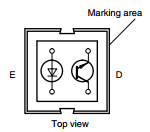
\includegraphics[scale=1.0]{./Graphics/CNY70-Diode}
\caption{billed af dioden og transisteren i CNY70}
\label{CNY70}
\end{wrapfigure}
Den refleksive optiske sensor som er valgt, hedder CNY70. Sensoren fylder $7x7x6$ mm og er placeret $0.2$ mm fra den overflade den operere på. \\
CNY70'eren er fastmonteret på undervognene af bilen, som vender ned mod banen.\\
\\
sensoren består af en diode og en fototransistor, da både diode og fototransistor vender ned mod banen, fungere den ved at lyset fra dioden reflektere i banen og fototransistoren opfangere det reflekterede lys og åbner alt efter hvor meget der bliver reflekteret. \\
\begin{wrapfigure}{r}{0.5\textwidth}
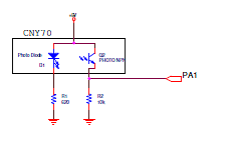
\includegraphics[scale=1.0]{./Graphics/Stregsensor_kredslob}
\caption{Det elektroniske kredsløb over stregsensoren}
\label{Stregsensor}
\end{wrapfigure}
Mørke farver absobere meget af lyset mens lyse farver reflektere dem. \\
(henvis til kredsløb for stregsensor)sensoren er forsynet med 5V, men kun når diodens stråler reflekteres åbner transistoren og udgangsspændingen på output-benet bliver højt.\\
Programmet til stregsensoren tjekker først på rising edge og registrere dette, så tjekker den for falling edge og registrere dette, microcontrolleren har nu dektekteret hele målstregen. \\



%\section{Elektromagnet}
\section{Elektromagnet}
Elektromagneten er lavet til at holde bilen på banen. ved at aktivere elektromagneten sving burde den optimere bilens evne til at holde sig på banen, ved højre hastighed end udens elektromagnet.

\subsection{Kernemateriale}
En vigtig faktor i fremstilling af elektromagneter er materialet. Ud fra materialet bestemmes, elektromagnetens magnetiake evne, hvori materialets permabiliteten bestemmer hvor det kan lede et magnetisk felt. Permeabiliteten kan deles op i tre underemner, ferromagnetisk, paramagnetisk og diamagnetisk. \\
I diamagnetiske materialer er magnetiseringen ekstremt lille og har en lineær BH-kurve. Ved paramagnetiske materialer er magnetiseringen ligeledes meget lille, men større end diamagnetiske materialer og ligeledes har materialet en lineær BH-kurve. Ferromagnetiske materialer har en stor magnetisering, den magnetiske effekt skyldes herved de uparede elektroner der forekommer i nogle metaller. Ferromagnetiske materialer har en logistisk stigende HB-kurve.\\
  \\
Ferromagnetisk materiale kan nu deles op i to undergrupper, blødt materiale og hårdt materiale. Blødt materiale er er karakteret ved høj permeabilitet, lille hysteresekurve med lille koerciv felt og lille kulstofindhold. Bløde materialer er ofte en legering af jern og silicium eller nikkel.\\
Hårdt materiale er karakteriseret ved mindre permeabilitet end blødt materiale, bred hysteresekurve, stort koerciv felt og højt kulstofindhold. Hårde materialer er ofte en legering af jern med kulstof, aluminium eller wolfram. 

\subsection{Prøvemagnet}
Som udgangspunkt er kernematerialet blevet antaget til at være stål da materialet er ferromagnetisk og hårdt. hvis der skulle laves en korrekt undersøgelse at kernematerialet ville det kræve en længere og meget tidskræven undersøgelse, derfor har dette kun været en overvejelse. \\
Næste overvejelse har været placering og form af elektromagnet. der er tre steder elektromagneten kan placeres på bilen, der er foran, bagpå eller under bilen.\\
Hverken trække eller skubbe elektromagneten er en effektiv løsning, det vil skabe uligevægt i bilen og flytte masse midtpunkt. ved en stærk elektomagnet vil man ændre friktions niveauet meget ved at have elektromagneten foran eller bagved, dvs. Hvis elektromagneten sidder bagpå vil der opstå meget friktion på baghjulene og mindre friktion på forhjulene.\\
Fluxspredning er en faktor der skal tages hensyn til når formen til elektromagneten laves, der vil altid være fluxspredning med formen kan være med til at reducere det betydligt. fluxlinjerne beværger sig fra nord til syd for fuldt udbytte af elektromagnet bør nord og syd pol befinde sig over skinnerne så fluxlinjerne løber med skinnerne. Hvis elektromagneten formes som en hestesko vil nord og syd pege ned mod skinnerne. for at undgå for meget fluxspredning bør luftgabet imellem nord og syd i hesteskoen være så stor som muligt, men da der er begrænset plads underbilen, kan lufgabet ikke blive særlig stort og en del kraft vil gå tabt i både fluxspredning og fluxfringing (se journal).\\
Nu da materialet er bestemt, placeringen og formen, skal antal vindinger bestemmes, da der er en maks bredde på pladsen under elektromagneten, vil der kun være plads til en 660 vindinger, før elektromagneten vil komme for tæt på banen, hvilket vil sige den ikke må komme tættere på end 2mm da bilen har affjedring og køre skævt i svingene. elektromagneten må ikke røre skinnerne da den enten vil gå i mætning eller kortslutte, så derfor er afstanden fra elektromagneten til skinnerne vigtigt.\\
\\
Test magneten er lavet ud fra forrige forhold og formlen for den magnetiske kraft i et luft gab (under idelle forhold) er givet ved:\\
\\
$F_{magn}(x)=-{\frac{B^{2}_{g}}{2\mu_{0}}}* {A_{j}}* (\frac{4x}{{\frac{l_{j}}{\mu_{r}}}+2x}-1) $
%$ {{\frac{4x}}{{frac{\l_{j}}{\mu_{r}}}}+2x}-1 $
\\
\\
Hvor $B_{g}$ er:
\\
\\
$ B_{g}(x)=\frac{\mu_{0}IN}{{\frac{l_{j}}{\mu_{r}}}+2x} $
\\
\\
Ud fra de overstående ligninger er kraften ideelt fundet til at være 1,309N. Virkeligt er den målt med en force sensor til at være 0,9367N. (henvis til journal) \\
Da 0,9367N er en meget lille kraft, bør de overvejes grundigt om elektromagneten vil blive en ulempe eller hjælp til bilen og hvor meget vil den lille kraft enlig kunne hjælpe med at forøge hastigheden i svingene. (henvis til peters afsnit)\\


% =====================================================================
%====== Primære afsnit ================================================
%======================================================================
\section{Måling af farten - Wheelspeed Sensor}
\label{fartmål}
I dette afsnit beskrives der hvordan en wheelspeed sensor udnyttes til at beregne farten bilen kører med. Der vil både blive beskrevet hardwaren til sensoren samt hvordan den softwaremæssigt bruger sensoren. Farten bliver brugt til at mappe banen samt kører med konstant hastighed. Disse funktioner vil blive beskrevet i afsnit \todo{indsæt afsnit for konstant hastighed og mapning}. \\

\subsection{Fart Hardware - TCST1230}
\label{fartmål_hardware}
Vi benytter TCST1230, som er en optisk sensor, til at lave en fotogate. Sensoren består af en fotocelle og en vifte med 16 blade på. Hjulet med vifterne sidder på motorens akse og hver gang aksen drejer en omgang vil den bryde fotosensorens lys XX gange. Hver gang lyset brydes så fås en puls fra fotosensoren som sendes videre til micro-controlleren. Dette er illustreret i figur \ref{wheelspeed3D} 

\begin{figure}[h!]
\center
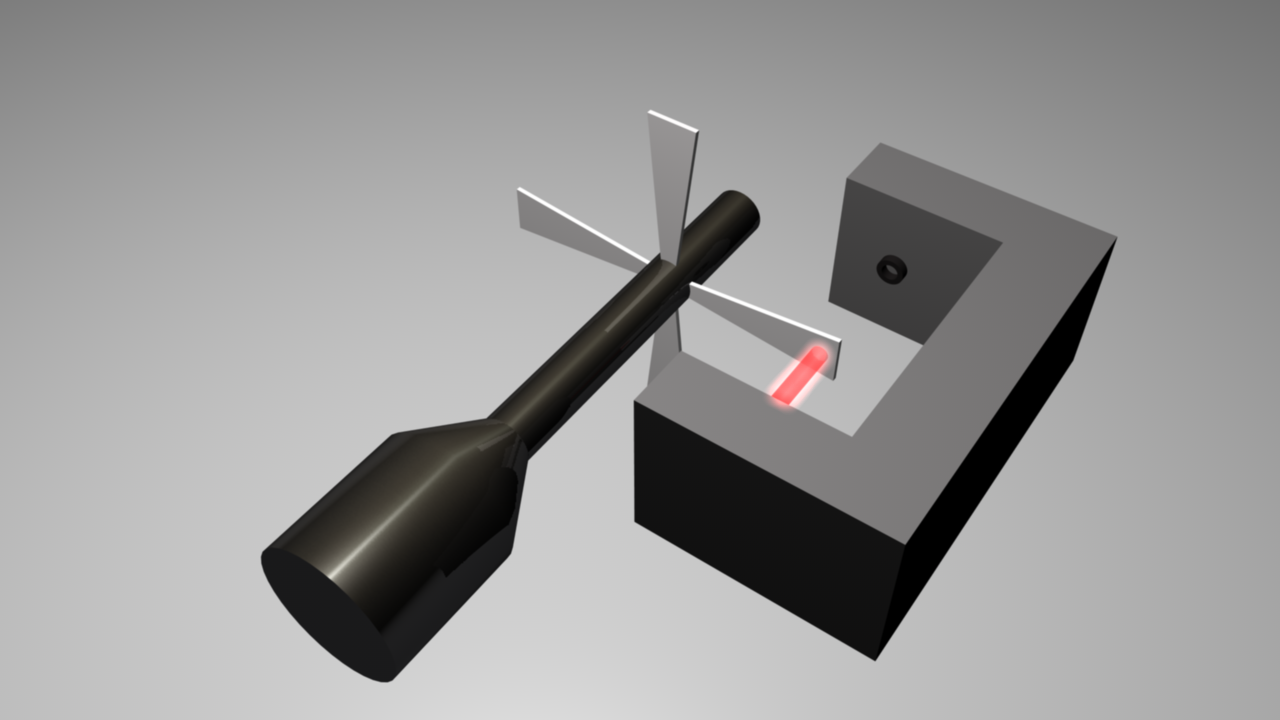
\includegraphics[scale=0.2]{./Graphics/Wheelspeed_D}
\caption{3D model af sensoren}
\label{wheelspeed3D}
\end{figure}

Efter test er der sat flere blade på viften da for at præcist at kunne bruge målingerne fra sensoren krævede det en højere opløsning. Dette fås ved at tilføje flere blade til viften så vi får flere pulses pr. omdrejning af aksen. Der er således nu så 4 blade på viften hvilket giver os 4 pulse pr. akse omdrejning. Dette svarer til 16,8 pulses pr. hjul omdrejning. \\
Se afsnit \ref{beregn_gearing} for udregningen af gearingen. \\
Dette giver en opløsning der er 4 gange bedre, end kun at have 1 vifte. \\
For bedre opløsning kunne der sættes flere vifter på, men kommer der for mange vifter på, vil det dog blive svært for sensoren at aflæse vifterne da deres mellemrum til sidst vil blive meget småt. Jo flere vifter der kommes på, jo sværere bliver det også at bygge ringen med vifterne. \\

Der bliver i dette tilfælde valgt at have 4 vifter da det kunne bygges forholdsvis let og det giver en opløsning der er høj nok til hvad vi ønskede. Ved blot 1 vifte kørte vi 2cm per omdrejning. Da vi ved hjulet kører 0,2381 omgange pr. motor omdrejning så kan længden den kører mellem hver puls udregnes ved at multiplicerer hjul omdrejninger med hjulets omkreds:
\begin{align*}
0,2381*8,5 = 2,02 cm
\end{align*}
Dette er ikke ret præcist da vi så kun kan aflæse længden/farten i intervaller af 2cm. Det blev så sat 4 vifter på og dette giver en præcision på:
\begin{align*}
(0,2381/4)* 8,5 = 0,51cm
\end{align*}
Dette er markant bedre da den nu kun kører 0,51cm før den får en puls og udregner længde og hastighed. Så der fås flere mindre intervaller der kan tjekkes og reageres på. \\ 

Som det kan ses på tegningen af kredsløbet i figur \ref{wheelspeedTegning} så er der sat nogle modstande og en kondensator på sensorens kredsløb. \\

\begin{figure}[h!]
\center
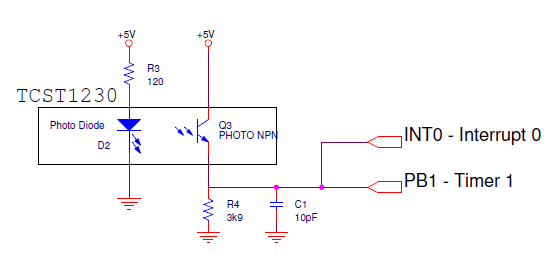
\includegraphics[scale=0.65]{./Graphics/TCST1230}
\caption{Kredsløbet til TCST1230 Sensoren}
\label{wheelspeedTegning}
\end{figure}

Modstanden R3 i figur \ref{wheelspeedTegning} er der for at sørge for at strømmen over dioden D2 ikke bliver højere end den kan tåle. Dioden kan nemlig kun klarer 30mA ifølge databladet. \todo{indsæt datablad}\\

Modstanden R4 virker som en pulldown modstand der sørger for at hive signalet langt nok ned, når fototransistoren ikke modtager lys, så der er logisk lavt signal. \\

Kondensatoren C1 benyttes til at sorterer små signaler fra. Hvis signalet ”hopper” frem og tilbage ved en overgang fra logisk lavt til logisk højt vil kondensatoren tage de små hurtige skift og sorterer dem fra. På denne måde fjernes en del af støjen.  
Der blev gennem oscilloskop observeret pral på sensoren ved TTL signal behandling. Der var benyttet en forkert metode til at opbygge sensoren på. Der var anvendt en struktur som forårsagede at diode spændingen over fototransistoren ikke kunne komme under 0.6V. Der blev derfor udarbejdet en anden struktur som set i databadet s. 3. \todo{TCST1230 s. 3} Modstanden benyttet til dioden blev udregnet vha. Ohms lov og ved at sætte strømmen lig 30mA. Dette resulterede i en modstand for R3 på 120 Ohm. \\

R4, som er pulldown modstanden, blev beregnet ved at kigge på figur 8 i databladet \todo{indsæt datablad}. Her blev modstanden udregnet til ca. 4K Ohm. Der anvendes her en 3.9K Ohm modstand \\

\subsection{Fart Software}
\label{fartmål_software}
Sensorens output er sat på ”PB1” og ”PD3” som går til ”Timer1” og ”INT0” i micro-controlleren. Så hver gang den får en puls så bliver timeren og interruptet triggeret. Timeren bliver benyttet til at finde længden den har kørt. Dette er beskrevet i afsnit \ref{afstandmål_software}. \\

Interruptet benyttes sammen med Timer0 til at finde farten. Timer 0 er sat op så den inkrementer hvert 0.000064 sekund. Hvilket svarer til den inkrementerer hvert 64. mikrosekund. Dette er sat ved at bruge en prescale på 1024. Da clock frekvensen på micro-processoren er 16MHz udregnes det således: \\
\begin{align*}
1/(16 000 000 / 1024) = 0,000064 sek = 64 mikrosekunder 
\end{align*}

Dette bruges for at finde tiden mellem pulses som kan benyttes som udtryk for farten. Timeren er ligeledes sat op så hvis der er overflow i Timer0 så kaldes et andet interrupt der blot nulstiller timeren og den fortsætter så. \\

Flowdiagrammet i figur \ref{fart_chart} viser processen hver gang Interruptet bliver kaldt. Hvilket sker hver gang sensoren sender en puls. \\

\begin{figure}[h!]
\center
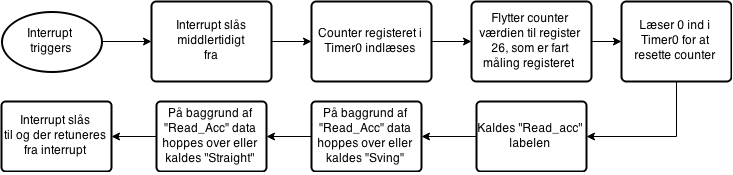
\includegraphics[scale=0.65]{./Graphics/fart_chart}
\caption{Flowchart af softwaren til måling af farten}
\label{fart_chart}
\end{figure}

Der slåes først interrupts fra globalt, for at dette interrupt ikke bliver afbrudt af et andet interrupt. Herefter indlæses den værdi tælleren er nået til. Denne værdi gemmes i registeret R26, som er vores ”målt fart” register. Så ligges der 0 ind i Timer0, for at nulstille den. På den måde får vi hvor mange gange der er gået 64 mikrosekunder på 1 puls. F.eks. hvis der går 10 optællinger mellem timer puls, så har bilen farten: 7,9 m/s. \\
Dette kan ses i lookup table i afsnit \todo{henvis til lookup table og sørg for table har korrekte enheder.}

Inden interruptet sluttes kaldes nogle labels der benyttes til at bestemme hvor på banen den er. Disse er beskrevet i afsnit XX. \todo{indsæt afsnit label} \\

Til sidst så slås interrupts til igen og der returneres til der koden var nået til, indtil næste interrupt bliver kaldt.  


\documentclass[11pt,a4paper,fleqn]{article} %Rapport, standard 11pt, A4
\usepackage[T1]{fontenc}
\usepackage[utf8]{inputenc}			%Muliggør æ,ø,å
\usepackage{lmodern}				%Skrifttype
\usepackage[danish]{babel}			%Styrer orddeling
\usepackage{graphicx}				%Billeder
\usepackage{epstopdf}				%Implementerer vectorgrafik
\usepackage{todonotes}				%Todo-kommentaterer
\usepackage{float}					%Håndterer floats
\usepackage{tabularx}				%Udvidede muligheder for tabeller
\usepackage{appendix}                
\usepackage{subcaption}				%Giver mulighed for subcaptions i billeder
\usepackage{wrapfig}				%For indsættelse af figur
\usepackage{blindtext}				%For indsættelse af blindtext
\usepackage{lastpage}               %For totale side antal
\usepackage{enumitem}
\setlist{nosep}                     %Or \setlist{noitemsep} to leave space around whole list
\usepackage{color}
\usepackage{xcolor}
\usepackage{placeins} %til float barrier								%Ændrer marginer
\usepackage[top=3cm, bottom=3cm, left=3.5cm, right=2.5cm]{geometry}
\usepackage{setspace}				%For ændring af linjeafstand
\usepackage{icomma}					%Fjerner mellemrum efter komma
\usepackage{pdfpages}


% =====================================================================
%====== Setting up author information==================================
%======================================================================

\title{\title}
\author{}
\date{}

\newcommand{\forfattere}{Peter Gilsaa, Mads Tilgaard Jensen, Eskild Andresen, \\
Sara Marie Gadgaard \& Frederik Mazur Andersen}
\newcommand{\titel}{Pole Position}
\newcommand{\korttitel}{Pole Position}
\newcommand{\afldato}{27. Maj 2015}
\newcommand{\fag}{PRO}
\newcommand{\klasse}{Autonome Robotter 2}


% =====================================================================
%====== Setting up Fancy Headers ======================================
%======================================================================
\usepackage{fancyhdr}
\pagestyle{fancy}
\renewcommand{\sectionmark}[1]{\markright{\thesection. \ #1}}
\lhead{\korttitel}
\chead{}
\rhead{\rightmark}
\lfoot{\forfattere}
\cfoot{}
\rfoot{Side \thepage\ af \pageref{LastPage}}
\renewcommand{\headrulewidth}{0.5pt}
\renewcommand{\footrulewidth}{0.5pt}

% øg tekst højden med 2 cm på alle sider
%\addtolength\textheight{2cm}
%\addtolength\topmargin{-1cm}
%\addtolength\marginparwidth{1.5cm}
%\addtolength\headheight{1.6pt}

\makeindex



\definecolor{sdu_grey}{RGB}{140,140,140}
\definecolor{sdu_blue}{RGB}{0,71,133}

% =====================================================================
%====== Setting up layout for chapters and force newpage ==============
%======================================================================									
\usepackage{titlesec}

\newcommand{\chapterbreak}{\clearpage}

\titleformat{\chapter}[display]	
	{\onehalfspacing \bfseries\Huge}
	{\filleft \color{sdu_grey} \LARGE Kapitel \thechapter}
	{1ex}
	{\titlerule
	\vspace{1ex}%
	\filright}
	[\vspace{1ex}%
	\titlerule]


\usepackage{hyperref}				%Til links
\usepackage{url}					%Til links
\hypersetup{pdfborder={0 0 0}}		%Fjerner bokse rundt om links
\usepackage[numbers]{natbib}		%Bibtex

\onehalfspacing
\bibliographystyle{plainnat}
\usepackage{multicol} %til at lave flere kolonner
\usepackage{graphicx}
\newcommand{\HRule}{\rule{\linewidth}{0.5mm}}
\setlength{\parindent}{0pt} %Ingen indhak
\usepackage[defaultlines=1,all]{nowidow}
\usepackage{amsmath}
\usepackage{gensymb}
\usepackage{listings} 
\begin{document}

\subsection{Måling af afstand}
\label{afstandmål}
I dette afsnit beskrives hvordan bilen måler hvor langt den er kørt. Her benyttes den samme sensor som bruges til udregning af farten der køres med. \\
Afstanden bilen har kørt bruges til at mappe banen som der kan læses nærmere om i afsnit XX \todo{indsæt afnist}

\subsubsection{Afstand Hardware - TCST1230}
\label{afstandmål_hardware}
Da sensoren er den samme som benyttes til måling af fart vil dens hardware ikke blive beskrevet her. Der henvises i stedet til afsnit \ref{fartmål_hardware} \\
Den eneste ændring på hardwaren er at sensores udgangssignal til micro-controlleren går på indgang ”PB1.”

\subsubsection{Afstand Software}
\label{afstandmål_software}
Hver gang sensoren sender en puls til ”PB1” på micro-controlleren så vil Timer1 inkrementer med en. Timer1 er valgt da det er en 16bit timer og derfor kan der køres XX meter før timeren giver overflow. Udregningen er som følger: 
\begin{align*}
udregning indsættes her
\end{align*}
\todo[inline]{fix udregning}
Dette er rigeligt til formålet, da efter hver lige strækning vil tælleren nulstilles.  \todo{indsæt tal} \\

Da der vides hvor mange pulses der går på en hjul omdrejning, nemlig 4.2, så kan der ved at tælle pulses udregnes hvor langt den har kørt. \todo{indsæt tal og henvis til journal} \\

Timer1 er opsat med en prescale der tager udgangspunkt i et ekstern input. Dette betyder at det eksterne signal benyttes som clock-frekvens med rising edge. Rising edge betyder at en periode tager udgangspunkt i signalet på vej op i stedet for på vej ned. 




\end{document}

\section{Motorstyring og bremsning}
For at finde den bedste måde at bremse på, er der lavet en test med tre scenarier. I alle tre scenarier er banen den samme. Banen består af 10 skinner. De første seks er tilsluttet strømforsyningen, mens de fire sidste er tilsluttet en kontakt så skinnerne kan frakobles strømforsyningen, kortsluttes eller strømmen vendes. Motoren er koblet direkte til banen, dvs. at den styres vha. strømforsyningen. I alle test er spændingsfaldet over motoren på 15 volt. Det hele filmes med højhastighedskamera. \\

I første test var de sidste fire skinner ikke tilsluttet til strømforsyningen ydermere var de ikke kortsluttet. Her viste testen at bilen skulle bruge mere en 70 cm. for at stoppe helt. \\
I anden test var de sidste fire skinner kortsluttet. Dvs. at motoren blev kortsluttet efter at have kørt på de seks første skinner. Her var bremselængden 67 cm. \\
I tredje test og sidste test løb strømmen den modsatte vej igennem motoren på de sidste fire skinner. Her var en væsentlig kortere bremselængde på kun 32 cm. \\

For at kunne vende strømmen i motoren er der placeret en h-bro. H-broen der anvendes er l293. Denne ic består af to h-broer, det er dog kun den ene som anvendes. H-broen er koblet til micro-controlleren med tre forbindelser. De tre forbindelser er enable, 1A og 2A. 

\begin{figure}[h!]
\center
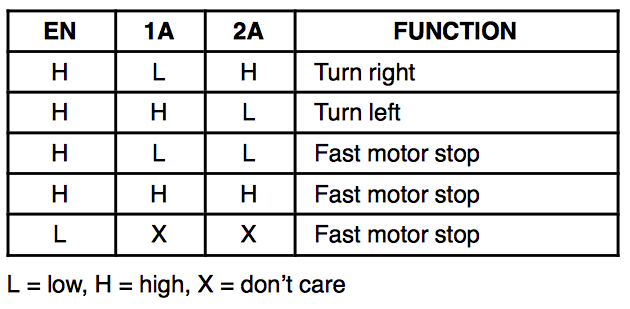
\includegraphics[scale=0.35]{./Graphics/h-bro_forbindelse.png}
\caption{H-broens 3 forbindelser og hvordan de kan sættes}
\label{hbro_forbindelse}
\end{figure}

PWM signalet fra micro-controlleren er koblet til 1A, mens enable og 2A er koblet til almindelige i/o pins. Som det ses vil et PWM signal medføre at motoren skifter mellem Fast motor stop og turn left. Dette er dog ikke et problem da man på lige strækninger kører med 100\% PWM hvilket svarer til at 1A konstant er høj. Derfor får man ikke lavere topfart i forhold til at køre uden h-bro. Dog vil det kræve et højere PWM signal for at holde samme fart i svingene i forhold til uden at bruge H-broen. Dette medvirker at bilen har et højere energiforbrug og mere spild energi, men der er intet krav om at bilen skal være effektiv. \todo{Skal dette med?} \\

Ved opbremsning ”slukkes” for PWM signalet og 2A sættes høj. Dette medfører at motoren prøver at køre den modsatte vej. Dette gøres kun kortvarigt så bilen kommer ned i en hastighed som gør at den ikke falder af i svingene. For at finde det optimale tidspunkt at bremse på er der lavet en række test og beregninger. Dette kan der læses nærmere om i afsnit \todo{afsnit udfyldes}.


\section{Sving}
\label{sving}
Bilen skal deltage i en racerløb, derfor er der blevet lagt vægt på at optimere bilens kørsel. 
For at kunne optimere omgangstiden skal der benyttes flere forskellige fysiske ligninger. Disse bruges til at finde bremsepunkterne og hastighedsgrænserne. Bilen er blevet udstyret med en omdrejningssensor således at hastigheden kan overvåges og benyttes løbende i ligningerne. \\

Før nogle af beregningerne kan laves skal massemidtpunktet i bilen findes. Dette gøres ved at hænge bilen i en snor, tage et billede og derefter hænges bilen op i et andet punkt. Stedet hvor fortsættelsen af snorene krydser hinanden indikerer massemidtpunktet, som vist i figur \ref{massemidtpunkt}. \\

\begin{wrapfigure}{r}{0.5\textwidth}
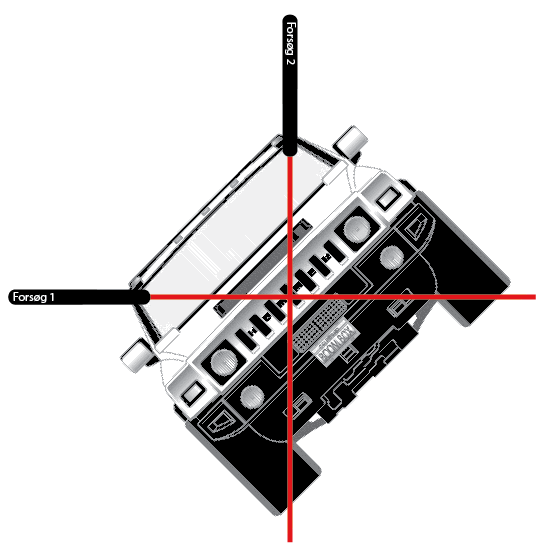
\includegraphics[scale=0.35]{./Graphics/massemidtpunkt.png}
\caption{Massemidtpunkt}
\label{massemidtpunkt}
\end{wrapfigure}

Efter at have fundet massemidtpunktet, måles afstanden fra punktet til banen. Denne distance benyttes herefter i en formel, der indikerer hvor hurtigt man kan køre i et sving.  \\

\( Fart(v) = (r*g*b/h)^\frac{1}{2} \), \\
r = radius,\\
g = tyngdekraft, \\
b = bilens bredde, \\
h = afstand mellem massemidtpunkt og banen. \\

For at optimere bilens fysiske egenskaber kan flere ting ændres. Opgaveformuleringen begrænser nogle muligheder såsom slibning af dæk, hvilket giver større overfladeareal og derved større friktion. \\

Derimod forbydes det ikke at justere bilens affjedring, hvilket giver ca. 3mm i massemidtpunktshøjde og derved højere teoretisk hastighed i svingene. Resultaterne for forskellige opsætninger kan ses i tabellen \ref{forskel_opsaat_result}. \\

\begin{table}[H]
\centering
\begin{tabular}{|l|l|l|}
\hline
Opsætning                      & Indre sving (m/s) & Ydre sving (m/s) \\ \hline
Standard u. perma,  u. elektro & 1,95              & 2,24             \\ \hline
Standard m. perma, u. elektro  & 2,64              & 3,03             \\ \hline
Standard u. perma, m. elektro  & 2,37              & 2,72             \\ \hline
Standard m. perma, m. elektro  & 2,87              & 3,30             \\ \hline
Sænket u. perma, u. elektro    & 2,12              & 2,43             \\ \hline
Sænket m. perma, u. elektro    & 2,86              & 3,28             \\ \hline
Sænket, u. perma, m. elektro   & 2,57              & 2,95             \\ \hline
Sænket, m. perma, m. elektro   & 3,12              & 3,58             \\ \hline
\end{tabular}
\caption{Forskellige opsætningers resultater}
\label{forskel_opsaat_result}
\end{table} 

Bredde af bil = \( 0,062m \), Svingradius Ydre = \( 0,33m \) \\
Svingradius Indre = \( 0,25m \), Tyngdekraft = \( 9,82m/s^2 \) \\
Permanent magnetkraft v. \( 2mm = 1,326N/8,1 m/s^2 \), \\
Elektromagnet v. \( 2mm = 0,9366N/4,7 m/s^2. \) \\  
Massemidtpunkthøjde = \( 0,02m \), Affjedring = \( [0;0,003m]. \) \\

Når det teoretiske maksimum er fundet skal resultatet implementeres i programmet. Da bilen ikke har et differentiale vil den decelerere i svinget. Derfor er det nødvendigt i programmet at tjekke den reelle hastighed bilen kører og sammenligne med den teoretiske. Dette gøres ved hjælp af omdrejningssensoren. Hvis der går for lang tid mellem pulsene øges bilens hastighed en smule. Hvis der går for kort tid mellem pulsene sænkes bilens hastighed en smule. Denne subrutine eksekveres gennem svinget således at hastigheden hele tiden reguleres til at være tættest på det teoretisk mulige. \\

\section{Bremse}
\label{bremse}
En stor del af optimeringen består i at finde det korrekte bremsepunkt. Jo senere der bremses jo hurtigere bliver omgangstiderne. For at finde disse bremsepunkter benyttes formlen: \\
\begin{align*}
V_f = V_i +2*a*d
\end{align*}
$V_f$ = maksimal fart i sving, $V_i$ = nuværende fart, a = deceleration(\(22.06m/s^2\)) og d = bremselængden. \\

Formlen benytter den maksimale teoretiske svinghastighed, bilens hastighed, deceleration og bremselængden. Da disse værdier ofte er kommatal, benyttes en lookup-tabel, som indeholder bremselængden som funktion af periodetiden fra omdrejningssensoren. \\

Lookup-tabellen i bilag \ref{lookup} tager udgangspunkt i en bestemt periodetid. Periodetiden benyttes til at udregnes hastigheden i $m/s$ og sættes ind i ovenstående formel. Konstanten A, er fundet ud fra et eksperiment, hvor bilen filmes mens den bremser. Videoen analyseres vha. programmet LoggerPro, som kan måle hastigheden og accelerationen. Ud fra disse værdier kan bremselængden findes. Denne måles i pulser, hvor det vides at 1 puls er lig med 0.005m. Dette er udregnet ud fra bilens gearing og hjulenes omkreds. Se afsnit \ref{beregn_gear} for beregninger.\\

Efter bilen har mappet banen benyttes lookup-tabellen til at finde det optimale bremsepunkt. Det gøres ved at tjekke omdrejningssensoren og sammenligne dennes værdi med værdierne i lookup-tabellen, for at finde bremselængden. Når afstanden til svinget er lig med bremselængde begynder bilen at bremse. Dette gøres ved at køre motoren baglæns indtil periodetiden i omdrejningssensoren er lig med den maksimale teoretiske periodetid for svinget. \\

Ud fra dette kan den optimale bremsedistance opnås og derved en hurtigere omgangstid. Da der kan være en del usikkerhed omkring testresultater osv. benyttes den optimale bremsedistance ikke i første omgang, da det kan resulterer i at bilen ryger af banen. I stedet øges bremsedistance i første omgang således at bilen med sikkerhed får sat en omgangstid. Herefter vil bilen i de følgende omgange nedsættes bremsedistancen indtil det teoretiske maksimum nås. \\


\section{Stregsensor}
På kørebanen til konkurrencen er der en hvis streg, som makere start. Det ønskes at kunne detektere dennne streg, for af vide hvornår bilen har kørt en omgang.\\
Til at dektektere start linjen, som er hvid skal den valgte sensor detekterer foreskellen mellem hvid og stort på banen.\\
 \\
Til det pågældende formål er en reflektiv optisk sensor blevet undersøgt og valgt. Den reflektive optiske sensore har fordelen at den er lille og fylder lidt.\\
\\

\subsection{CNY70}
\begin{wrapfigure}{r}{0.5\textwidth}
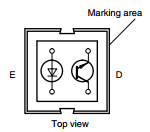
\includegraphics[scale=1.0]{./Graphics/CNY70-Diode}
\caption{billed af dioden og transisteren i CNY70}
\label{CNY70}
\end{wrapfigure}
Den refleksive optiske sensor som er valgt, hedder CNY70. Sensoren fylder $7x7x6$ mm og er placeret $0.2$ mm fra den overflade den operere på. \\
CNY70'eren er fastmonteret på undervognene af bilen, som vender ned mod banen.\\
\\
sensoren består af en diode og en fototransistor, da både diode og fototransistor vender ned mod banen, fungere den ved at lyset fra dioden reflektere i banen og fototransistoren opfangere det reflekterede lys og åbner alt efter hvor meget der bliver reflekteret. \\
\begin{wrapfigure}{r}{0.5\textwidth}
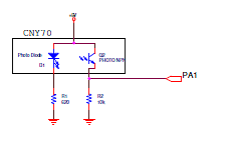
\includegraphics[scale=1.0]{./Graphics/Stregsensor_kredslob}
\caption{Det elektroniske kredsløb over stregsensoren}
\label{Stregsensor}
\end{wrapfigure}
Mørke farver absobere meget af lyset mens lyse farver reflektere dem. \\
(henvis til kredsløb for stregsensor)sensoren er forsynet med 5V, men kun når diodens stråler reflekteres åbner transistoren og udgangsspændingen på output-benet bliver højt.\\
Programmet til stregsensoren tjekker først på rising edge og registrere dette, så tjekker den for falling edge og registrere dette, microcontrolleren har nu dektekteret hele målstregen. \\



\section{Elektromagnet}
Elektromagneten er lavet til at holde bilen på banen. ved at aktivere elektromagneten sving burde den optimere bilens evne til at holde sig på banen, ved højre hastighed end udens elektromagnet.

\subsection{Kernemateriale}
En vigtig faktor i fremstilling af elektromagneter er materialet. Ud fra materialet bestemmes, elektromagnetens magnetiake evne, hvori materialets permabiliteten bestemmer hvor det kan lede et magnetisk felt. Permeabiliteten kan deles op i tre underemner, ferromagnetisk, paramagnetisk og diamagnetisk. \\
I diamagnetiske materialer er magnetiseringen ekstremt lille og har en lineær BH-kurve. Ved paramagnetiske materialer er magnetiseringen ligeledes meget lille, men større end diamagnetiske materialer og ligeledes har materialet en lineær BH-kurve. Ferromagnetiske materialer har en stor magnetisering, den magnetiske effekt skyldes herved de uparede elektroner der forekommer i nogle metaller. Ferromagnetiske materialer har en logistisk stigende HB-kurve.\\
  \\
Ferromagnetisk materiale kan nu deles op i to undergrupper, blødt materiale og hårdt materiale. Blødt materiale er er karakteret ved høj permeabilitet, lille hysteresekurve med lille koerciv felt og lille kulstofindhold. Bløde materialer er ofte en legering af jern og silicium eller nikkel.\\
Hårdt materiale er karakteriseret ved mindre permeabilitet end blødt materiale, bred hysteresekurve, stort koerciv felt og højt kulstofindhold. Hårde materialer er ofte en legering af jern med kulstof, aluminium eller wolfram. 

\subsection{Prøvemagnet}
Som udgangspunkt er kernematerialet blevet antaget til at være stål da materialet er ferromagnetisk og hårdt. hvis der skulle laves en korrekt undersøgelse at kernematerialet ville det kræve en længere og meget tidskræven undersøgelse, derfor har dette kun været en overvejelse. \\
Næste overvejelse har været placering og form af elektromagnet. der er tre steder elektromagneten kan placeres på bilen, der er foran, bagpå eller under bilen.\\
Hverken trække eller skubbe elektromagneten er en effektiv løsning, det vil skabe uligevægt i bilen og flytte masse midtpunkt. ved en stærk elektomagnet vil man ændre friktions niveauet meget ved at have elektromagneten foran eller bagved, dvs. Hvis elektromagneten sidder bagpå vil der opstå meget friktion på baghjulene og mindre friktion på forhjulene.\\
Fluxspredning er en faktor der skal tages hensyn til når formen til elektromagneten laves, der vil altid være fluxspredning med formen kan være med til at reducere det betydligt. fluxlinjerne beværger sig fra nord til syd for fuldt udbytte af elektromagnet bør nord og syd pol befinde sig over skinnerne så fluxlinjerne løber med skinnerne. Hvis elektromagneten formes som en hestesko vil nord og syd pege ned mod skinnerne. for at undgå for meget fluxspredning bør luftgabet imellem nord og syd i hesteskoen være så stor som muligt, men da der er begrænset plads underbilen, kan lufgabet ikke blive særlig stort og en del kraft vil gå tabt i både fluxspredning og fluxfringing (se journal).\\
Nu da materialet er bestemt, placeringen og formen, skal antal vindinger bestemmes, da der er en maks bredde på pladsen under elektromagneten, vil der kun være plads til en 660 vindinger, før elektromagneten vil komme for tæt på banen, hvilket vil sige den ikke må komme tættere på end 2mm da bilen har affjedring og køre skævt i svingene. elektromagneten må ikke røre skinnerne da den enten vil gå i mætning eller kortslutte, så derfor er afstanden fra elektromagneten til skinnerne vigtigt.\\
\\
Test magneten er lavet ud fra forrige forhold og formlen for den magnetiske kraft i et luft gab (under idelle forhold) er givet ved:\\
\\
$F_{magn}(x)=-{\frac{B^{2}_{g}}{2\mu_{0}}}* {A_{j}}* (\frac{4x}{{\frac{l_{j}}{\mu_{r}}}+2x}-1) $
%$ {{\frac{4x}}{{frac{\l_{j}}{\mu_{r}}}}+2x}-1 $
\\
\\
Hvor $B_{g}$ er:
\\
\\
$ B_{g}(x)=\frac{\mu_{0}IN}{{\frac{l_{j}}{\mu_{r}}}+2x} $
\\
\\
Ud fra de overstående ligninger er kraften ideelt fundet til at være 1,309N. Virkeligt er den målt med en force sensor til at være 0,9367N. (henvis til journal) \\
Da 0,9367N er en meget lille kraft, bør de overvejes grundigt om elektromagneten vil blive en ulempe eller hjælp til bilen og hvor meget vil den lille kraft enlig kunne hjælpe med at forøge hastigheden i svingene. (henvis til peters afsnit)\\



\section{Kommunikation mellem computer og bil}
\label{kom_bil}

I opgaveformuleringen stilles visse krav til bilens kommunikation. Det skal være muligt at sende beskeder fra f.eks. en computer til bilen. Denne kommunikation skal som minimum kunne sætte bilens hastighed, og stoppe den igen. For at gøre det skal kommunikationen leve op til en protokol, som er dikteret i opgaveoplægget. Protokollen nødvendiggør at der skal sendes tre bytes hver gang. De tre bytes som sendes af sted har hver deres funktion. Den første byte beskriver typen af besked, anden byte er kommandoen, mens tredje byte er data som skal overføres til bilen. Protokollen kræver kun tre forskellige typer af beskeder, disse tre typer kan ses herunder.

\begin{table}[h]
\begin{tabular}{|c|c|l|}
\hline
Hex Værdi & Type  & \multicolumn{1}{c|}{Bemærkning}                                   \\ \hline
0x55      & SET   & Bruges til at sætte/aktivere en værdi i bilen. Kræver intet svar. \\ \hline
0xAA      & GET   & Bruges til at hente en værdi i bilen.                             \\ \hline
0xBB      & REPLY & Er et svar på en GET besked.                                      \\ \hline
\end{tabular}
\caption{Forskellige typer af beskeder}
\label{forskel_besked}
\end{table}

Typen er efterfulgt af en kommando. Det kræves at der minimum er start og stop kommandoer. Protokollen er dog blevet udvidet så den indeholder en del flere kommandoer. Dette er gjort så det i højere grad er lettere at lave test på bilen. F.eks. er det muligt at måle bilens fart eller accelerationen vinkelret på bilen. I det følgende skema kan de forskellige kommandoer ses.

\begin{table}[h]
\center
\begin{tabular}{|c|c|l|}
\hline
Hex Værdi & Type     &  \multicolumn{1}{c|}{Bemærkning}                                     \\ \hline
0x10      & Start    & Dataværdi mellem 0 og 100                      \\ \hline
0x11      & Stop     & Dataværdi er underordnet                       \\ \hline
0x12      & Register & Dataværdi mellem 0 og 25                       \\ \hline
0x13      & MapH     & MSB af banelængden                             \\ \hline
0x14      & MapL     & LSB af banelængden                             \\ \hline
0x15      & Acc      & Returnerer en værdi mellem 0 og 255            \\ \hline
0x16      & Speed    & Periode tiden fra Sensor                       \\ \hline
0xBB      & Error    & Sendes tilbage 3 gange ved fejl                \\ \hline
\end{tabular}
\caption{Forskellige kommandoer}
\label{forskel_kommando}
\end{table}

\textbf{Start} kommandoen bruges til at sætte bilens hastighed. Hastigheden sendes som et procenttal mellem 0-100\%. Dette tal skal konverteres til hex inden afsendelse. Hexværdien skal derfor være mellem 0x00-0x64. Hvis en værdi højere end 0x64 sendes, skal bilen ignorere beskeden, da der er tale om en ugyldig besked. \\

\textbf{Stop} kommandoen bruges til at stoppe bilen. Det er ikke afgørende hvilken data værdi som sendes af sted med stop kommandoen, dog skal der i alt sendes tre bytes af sted, da bilen forventer dette. Man kan således ikke blot sende 0x55 0x11. \\ 

\textbf{Register} kommandoen er indført så der lettere kan udføres debugging. Kommandoen efterfølges med en værdi mellem 20 og 25. Hvis der f.eks. skrives ”Get Register 25” svarer bilen tilbage med Reply Register og værdien i register 25. I dette tilfælde befinder bilens fart sig i register 25. Dette muliggør at man f.eks. kan tjekke om bilen har modtaget den set besked som skulle starte bilen. \\

\textbf{MapH} og \textbf{MapL} er tælleregistrer. Disse to registre udgør tilsammen et 16-bit register som bruges til at tælle antal pulses fra wheelspeedsensoren. På denne måde er det muligt at måle hvor langt bilen har kørt. Når den hvide linje krydses sendes værdierne fra disse registre til f.eks. computeren, herefter nulstilles registrene. Dette blev implementeret så der kunne laves test på hvor konsistent wheelspeedsensoren er. Det 16-bit register tillader en teoretisk max bane længde på……………. Dette kan der læses nærmere om i bilag \todo{Hvilket bilag?} \\

\textbf{Acc} kommandoen bruges til at aflæse ADC’en som er koblet til accelerometeret. På lige strækninger er denne værdi omkring 128…………………. \\

\textbf{Speed} kommandoen anvendes hvis man ønsker at måle bilens fart. Denne kommando er blevet implementeret for at kunne debugge i den del af programmet som sørger for at bilen kører med konstant hastighed. ………………………. \\


\textbf{Error} er svaret på alle ikke kendte beskeder. Dvs. hvis man sender en ikke gyldig kommando til bilen, så svarer den tilbage med 0xBB 0xBB 0xBB. \\

ATMega32 chippen indeholder et USART modul. USART er et initialord for universal synchronous/asynchronous receiver/transmitter. I dette projekt bruges modulet dog bare som UART(universal asynchronous receiver/transmitter). Fordelen ved at benytte asynkron dataoverførsel er at det ikke er nødvendigt med et fælles kloksignal. Da der ikke er et fælles kloksignal skal hver dataoverførsel indledes med et startbit, efterfulgt af 5-9 data bits og beskeden skal slutte med 0-2 stopbits. Det er også muligt at afsende et parity bit. Parity bittet kan bruges til at tjekke om der er fejl i det data som er modtaget. I dette projekt anvendes et start bit, 8 data bits og 1 stop bit. De otte data bits sendes af sted som et hex tal mellem 0x00 og 0xFF. Beskederne til bilen sendes trådløs fra f.eks. en computer via bluetooth. \\


%\input{Include/mapning}

% =====================================================================
%====== Konklusion ====================================================
%======================================================================
%\include{Konklusion}

%\section{Litteraturliste}
\section{Litteraturliste}
\subsection{Kilder}
\begin{enumerate}
\item Atmel, 8-bit AVR: Instruction Set.(PDF), \\
\url{https://e-learn.sdu.dk/bbcswebdav/pid-3951952-dt-content-rid-5381354_2/courses/RB-AUR2-U1-1-F15/AVR\%20Instruction\%20Set\%281\%29.pdf} 26/05-2015
\item Muhammed Ali Mazidi, Sarmad Naimi og Sepehr Naimi: AVR Microcontroller and Embedded System: Using Assembly and C, 2011
\item Schoolphysics: Circular Motion, Cars on flat track, \\
\url{http://www.schoolphysics.co.uk/age16-19/Mechanics/Circular\%20motion/text/Cars_cornering/index.html} 20/05-2015.
\item Søren Hassing og René Skov Hansen: Elektrofysik (E-ANA 1), supplerende noter.(PDF), Efterår 1997
\end{enumerate}

\subsection{Datasheets}
\begin{enumerate}
\item Atmega32A - Atmel, \\
\url{https://e-learn.sdu.dk/bbcswebdav/pid-3951952-dt-content-rid-5381352_2/courses/RB-AUR2-U1-1-F15/ATmega32A\%20datasheet\%281\%29.pdf} 26/05-2015
\item CNY70 - Vishay, \\
\url{http://www.vishay.com/docs/83751/cny70.pdf} 26/05-2015
\item L293 - Texas, \\
\url{http://users.ece.utexas.edu/~valvano/Datasheets/L293d.pdf} 26/05-2015
\item MMA1270KEG - Freescale Semiconductors, \\
\url{http://cache.freescale.com/files/sensors/doc/data_sheet/MMA1270KEG.pdf} 26/05-2015
\item TCST1230 - Vishay, \\
\url{http://www.vishay.com/docs/83765/tcst1230.pdf} 26/05-2015
\end{enumerate}


%\section{Ordliste}
\section{Ordliste}
\label{ordliste}
\begin{itemize}
\item Falling edge: Overgang fra højt til lavt.
\item HB-kurve: en hysteresekurve
\item Koerciv kraft: den modstående magnetisk intensitet.
\item Rising edge: Overgang fra lavt til højt.
\item RPM: Rounds pr. minut
\item RPS: Rounds pr. sekund 
\item PPS: Pulses pr. sekund
\item Pulldown modstand: Signalet holdet lavt pga. pulldown modstand. 
\end{itemize}


%\section{Symbolliste}
\section{Symbolliste}

\begin{tabular}{|c|c|c|}
\hline 
Symbol & Betydning & Enhed \\ 
\hline 
B-felt & Flux densitet & T \\ 
\hline 
H-felt & Felt styrke & $\frac{A}{m}$\\
\hline 
$\mu_{r}$ & Relativ permeabilitet & - \\
\hline 
$\mu_{0}$ & Permeabilitetskonstant & $\frac{H}{m}$\\
\hline 
$F_{magn}$ & Magnetisk kraft & N \\
\hline
$\epsilon$ & Diaelektrisk konstant & - \\
\hline
$f$ & Frekvens & Hz \\
\hline
$B_{g}$ & Flux densitet i luftgab  & T \\
\hline
$ B_{j}$ & Flux densitet i jern & T \\
\hline
$ H_{j} $ & Felt styrke i jern & $\frac{A}{m}$ \\
\hline
$ H_{g} $ & Felt styrke i luftgab & $\frac{A}{m}$ \\
\hline
$ l_{j} $ & Middelvejs længde & m \\
\hline
x & Lufgabs højde	& m \\
\hline
I & Strøm & A \\
\hline
N & Viklinger & - \\
\hline
$ A_{j} $ & Tværsnits areal & $ m^2 $ \\
\hline
$ U_{B} $ & Magnetisk potentiel energi & J \\
\hline
\end{tabular} 


\newpage
\section{Bilag}
\input{Include/Elektromagnet-kraftmåling}

\documentclass[11pt,a4paper,fleqn]{article} %Rapport, standard 11pt, A4
\usepackage[T1]{fontenc}
\usepackage[utf8]{inputenc}			%Muliggør æ,ø,å
\usepackage{lmodern}				%Skrifttype
\usepackage[danish]{babel}			%Styrer orddeling
\usepackage{graphicx}				%Billeder
\usepackage{epstopdf}				%Implementerer vectorgrafik
\usepackage{todonotes}				%Todo-kommentaterer
\usepackage{float}					%Håndterer floats
\usepackage{tabularx}				%Udvidede muligheder for tabeller
\usepackage{appendix}                
\usepackage{subcaption}				%Giver mulighed for subcaptions i billeder
\usepackage{wrapfig}				%For indsættelse af figur
\usepackage{blindtext}				%For indsættelse af blindtext
\usepackage{lastpage}               %For totale side antal
\usepackage{enumitem}
\setlist{nosep}                     %Or \setlist{noitemsep} to leave space around whole list
\usepackage{color}
\usepackage{xcolor}
\usepackage{placeins} %til float barrier								%Ændrer marginer
\usepackage[top=3cm, bottom=3cm, left=3.5cm, right=2.5cm]{geometry}
\usepackage{setspace}				%For ændring af linjeafstand
\usepackage{icomma}					%Fjerner mellemrum efter komma
\usepackage{pdfpages}


% =====================================================================
%====== Setting up author information==================================
%======================================================================

\title{\title}
\author{}
\date{}

\newcommand{\forfattere}{Peter Gilsaa, Mads Tilgaard Jensen, Eskild Andresen, \\
Sara Marie Gadgaard \& Frederik Mazur Andersen}
\newcommand{\titel}{Pole Position}
\newcommand{\korttitel}{Pole Position}
\newcommand{\afldato}{27. Maj 2015}
\newcommand{\fag}{PRO}
\newcommand{\klasse}{Autonome Robotter 2}


% =====================================================================
%====== Setting up Fancy Headers ======================================
%======================================================================
\usepackage{fancyhdr}
\pagestyle{fancy}
\renewcommand{\sectionmark}[1]{\markright{\thesection. \ #1}}
\lhead{\korttitel}
\chead{}
\rhead{\rightmark}
\lfoot{\forfattere}
\cfoot{}
\rfoot{Side \thepage\ af \pageref{LastPage}}
\renewcommand{\headrulewidth}{0.5pt}
\renewcommand{\footrulewidth}{0.5pt}

% øg tekst højden med 2 cm på alle sider
%\addtolength\textheight{2cm}
%\addtolength\topmargin{-1cm}
%\addtolength\marginparwidth{1.5cm}
%\addtolength\headheight{1.6pt}

\makeindex



\definecolor{sdu_grey}{RGB}{140,140,140}
\definecolor{sdu_blue}{RGB}{0,71,133}

% =====================================================================
%====== Setting up layout for chapters and force newpage ==============
%======================================================================									
\usepackage{titlesec}

\newcommand{\chapterbreak}{\clearpage}

\titleformat{\chapter}[display]	
	{\onehalfspacing \bfseries\Huge}
	{\filleft \color{sdu_grey} \LARGE Kapitel \thechapter}
	{1ex}
	{\titlerule
	\vspace{1ex}%
	\filright}
	[\vspace{1ex}%
	\titlerule]


\usepackage{hyperref}				%Til links
\usepackage{url}					%Til links
\hypersetup{pdfborder={0 0 0}}		%Fjerner bokse rundt om links
\usepackage[numbers]{natbib}		%Bibtex

\onehalfspacing
\bibliographystyle{plainnat}
\usepackage{multicol} %til at lave flere kolonner
\usepackage{graphicx}
\newcommand{\HRule}{\rule{\linewidth}{0.5mm}}
\setlength{\parindent}{0pt} %Ingen indhak
\usepackage[defaultlines=1,all]{nowidow}
\usepackage{amsmath}
\usepackage{gensymb}
\usepackage{listings} 
\begin{document}

\section{Beregning af gearing}
\label{beregn_gear}

For at udregne hvor langt hjulet drejer på en puls og hvor mange pulse der skal til for at hjulet drejer en hel omgang skal gearing udregnes. \\
Dette udregnes ved at kigger på de 2 tandhjul som er henholdsvis gear 1 og 2. Der kigges på begge tandhjul og deres tænder tælles. Ved at dividerer værdierne fås forholdet mellem tandhjulene. \\
Dette har givet følgende forhold:
\begin{align*}
Gear1 = 10 / 14 = 0,7143 \\
Gear2 = 9 / 127 = 0,3333
\end{align*}
Ligges gearene sammen:
\begin{align*}
Gear1*Gear2 = 0,7143 * 0,3333 = 0,2381
\end{align*}

Dette betyder at når motoren har drejet en omgang så har hjulet drejet \(0,2381\) omgange.
Når sensoren giver en puls, har hjulet derfor kørt: \(\frac{0,2381}{4} = 0,0595\) \\
Da hjulet er 8.5 cm i omkreds så svarer 1 puls til: \(0,0595*8,5 = 0,50595\)

\subsection{Periode tid ved 4 m/s}
\label{periode_4ms}
Her udregnes periode tiden for signalet ved en hastighed på 4 m/s:
\begin{align*}
\frac{4m/s}{0,085m} = 47,1 RPS
\end{align*}

Når hjulet har kørt en omgang har motoren altså kørt:
\begin{align*}
(\frac{27}{9}) * (\frac{14}{10}) = 4,2
\end{align*}

Så motoren kører: \(47,1 RPS * 4,2 = 197,82 RPS = 11869,2 RPM \) \\
Så der er: \(197,82 RPS *4 = 791,28 PPS \) \\
\(1/791,28 = 0,001265 sekunder \) \\
Dette giver altså en periode tid på: \(1,26 ms\)

\end{document}

\subsection{Lookup Table - Bremse Værdi}
\label{lookup}
\todo{lav en beregning fra tid til m/s, og forklar hvad enhed tiden er}

\begin{table}[h]
\centering
\begin{tabular}{|c|c|c|c|}
\hline
\multicolumn{1}{|l|}{Tid mellem pulses} & \multicolumn{1}{l|}{Hastighed(m/s)} & \multicolumn{1}{l|}{Bremselængde(m)} & \multicolumn{1}{l|}{Bremselængde(pulse)} \\ \hline
10                                      & 7,906                               & 0,145596591                          & 29                                       \\ \hline
11                                      & 7,188                               & 0,129261364                          & 26                                       \\ \hline
12                                      & 6,589                               & 0,115648674                          & 23                                       \\ \hline
13                                      & 6,082                               & 0,104130245                          & 21                                       \\ \hline
14                                      & 5,647                               & 0,094257305                          & 19                                       \\ \hline
15                                      & 5,271                               & 0,085700758                          & 17                                       \\ \hline
16                                      & 4,941                               & 0,078213778                          & 15                                       \\ \hline
17                                      & 4,651                               & 0,07160762                           & 14                                       \\ \hline
18                                      & 4,392                               & 0,06573548                           & 13                                       \\ \hline
19                                      & 4,161                               & 0,060481459                          & 12                                       \\ \hline
20                                      & 3,953                               & 0,055752841                          & 11                                       \\ \hline
21                                      & 3,765                               & 0,051474567                          & 10                                       \\ \hline
22                                      & 3,594                               & 0,047585227                          & 9                                        \\ \hline
23                                      & 3,438                               & 0,044034091                          & 9                                        \\ \hline
24                                      & 3,294                               & 0,040778883                          & 8                                        \\ \hline
25                                      & 3,163                               & 0,037784091                          & 7                                        \\ \hline
26                                      & 3,041                               & 0,035019668                          & 7                                        \\ \hline
27                                      & 2,928                               & 0,032460017                          & 6                                        \\ \hline
28                                      & 2,824                               & 0,030083198                          & 6                                        \\ \hline
29                                      & 2,726                               & 0,027870298                          & 6                                        \\ \hline
30                                      & 2,635                               & 0,025804924                          & 5                                        \\ \hline
31                                      & 2,550                               & 0,023872801                          & 5                                        \\ \hline
32                                      & 2,471                               & 0,022061435                          & 4                                        \\ \hline
33                                      & 2,396                               & 0,020359848                          & 4                                        \\ \hline
34                                      & 2,325                               & 0,018758356                          & 4                                        \\ \hline
35                                      & 2,259                               & 0,017248377                          & 3                                        \\ \hline
36                                      & 2,196                               & 0,015822285                          & 3                                        \\ \hline
37                                      & 2,137                               & 0,01447328                           & 3                                        \\ \hline
38                                      & 2,081                               & 0,013195275                          & 3                                        \\ \hline
39                                      & 2,027                               & 0,011982809                          & 2                                        \\ \hline
40                                      & 1,977                               & 0,010830966                          & 2                                        \\ \hline
41                                      & 1,928                               & 0,00973531                           & 2                                        \\ \hline
42                                      & 1,882                               & 0,008691829                          & 2                                        \\ \hline
43                                      & 1,839                               & 0,007696882                          & 2                                        \\ \hline
44                                      & 1,797                               & 0,006747159                          & 1                                        \\ \hline
45                                      & 1,757                               & 0,005839646                          & 1                                        \\ \hline
46                                      & 1,719                               & 0,004971591                          & 1                                        \\ \hline
47                                      & 1,682                               & 0,004140474                          & 1                                        \\ \hline
48                                      & 1,647                               & 0,003343987                          & 1                                        \\ \hline
49                                      & 1,614                               & 0,002580009                          & 1                                        \\ \hline
50                                      & 1,581                               & 0,001846591                          & 0                                        \\ \hline
\end{tabular}
\caption{Table med udregnede værdier for hurtig brug}
\label{lookuptable}
\end{table}

\end{document}